\documentclass[12pt, a4paper, twoside]{article}

%% Preamble
\usepackage{pdfpages}           % Para incluir PDFs
\usepackage{graphicx}           % Para gráficos
\usepackage{subfiles}           % Para manejar subarchivos
\usepackage{hyperref}           % Para enlaces
\usepackage{listings}           % Para código fuente (ajusta lenguaje)
\usepackage[style=numeric]{biblatex}  % Carga de biblatex con el estilo numérico

\addbibresource{references.bib}  % Archivo de bibliografía (asegúrate de que el nombre del archivo sea correcto)


\usepackage{geometry}           % Para ajustar márgenes

% Ajustes de márgenes
\geometry{
	left=3cm,       % Margen izquierdo
	right=3cm,      % Margen derecho
	top=2.5cm,      % Margen superior
	bottom=2.5cm,   % Margen inferior
	headheight=15pt, % Altura del encabezado
	twoside          % Para documentos a dos caras
}


\graphicspath{{images/}{../images/}} % Ruta para imágenes

\begin{document}
	
	%% Cover
	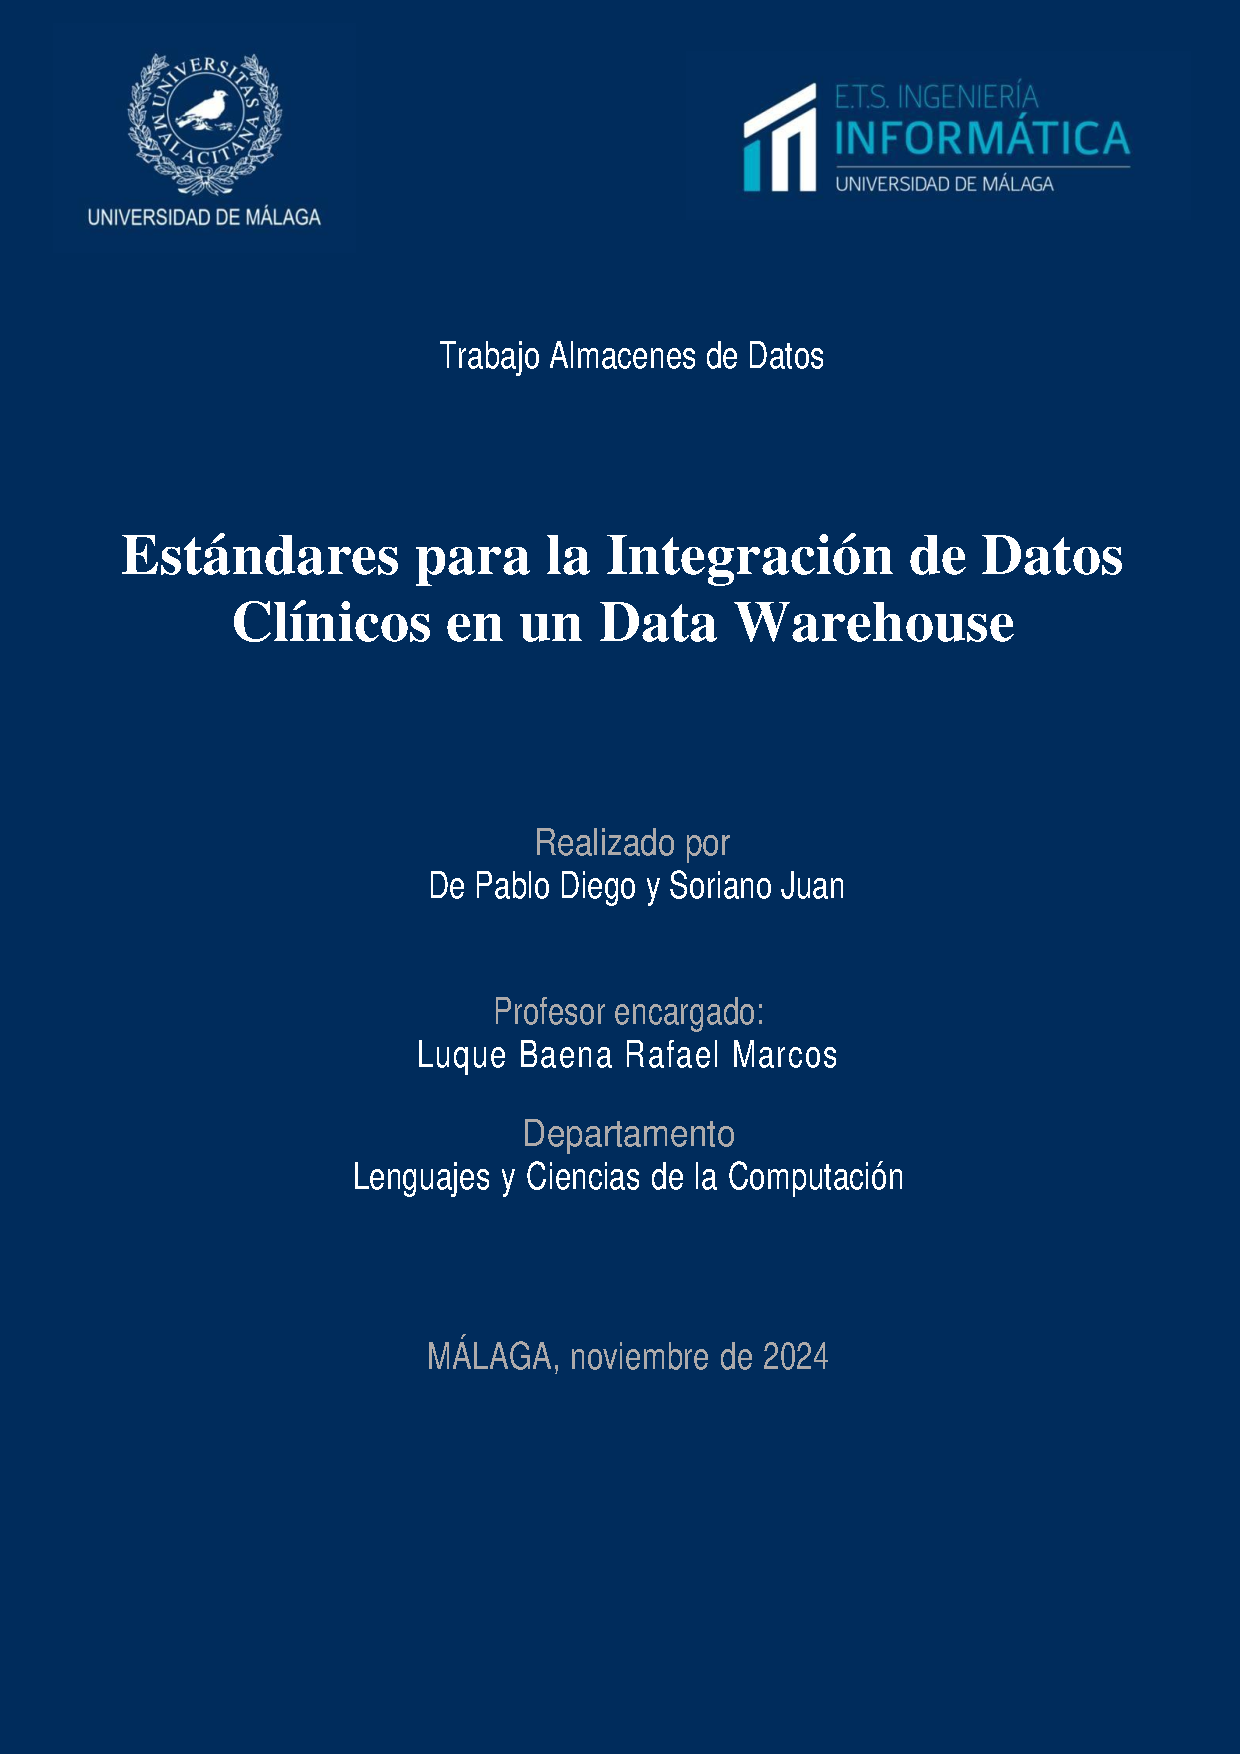
\includepdf[noautoscale=true, width=\paperwidth]{cover.pdf}
	
	%% Title
	\clearpage
	\setcounter{page}{1}
	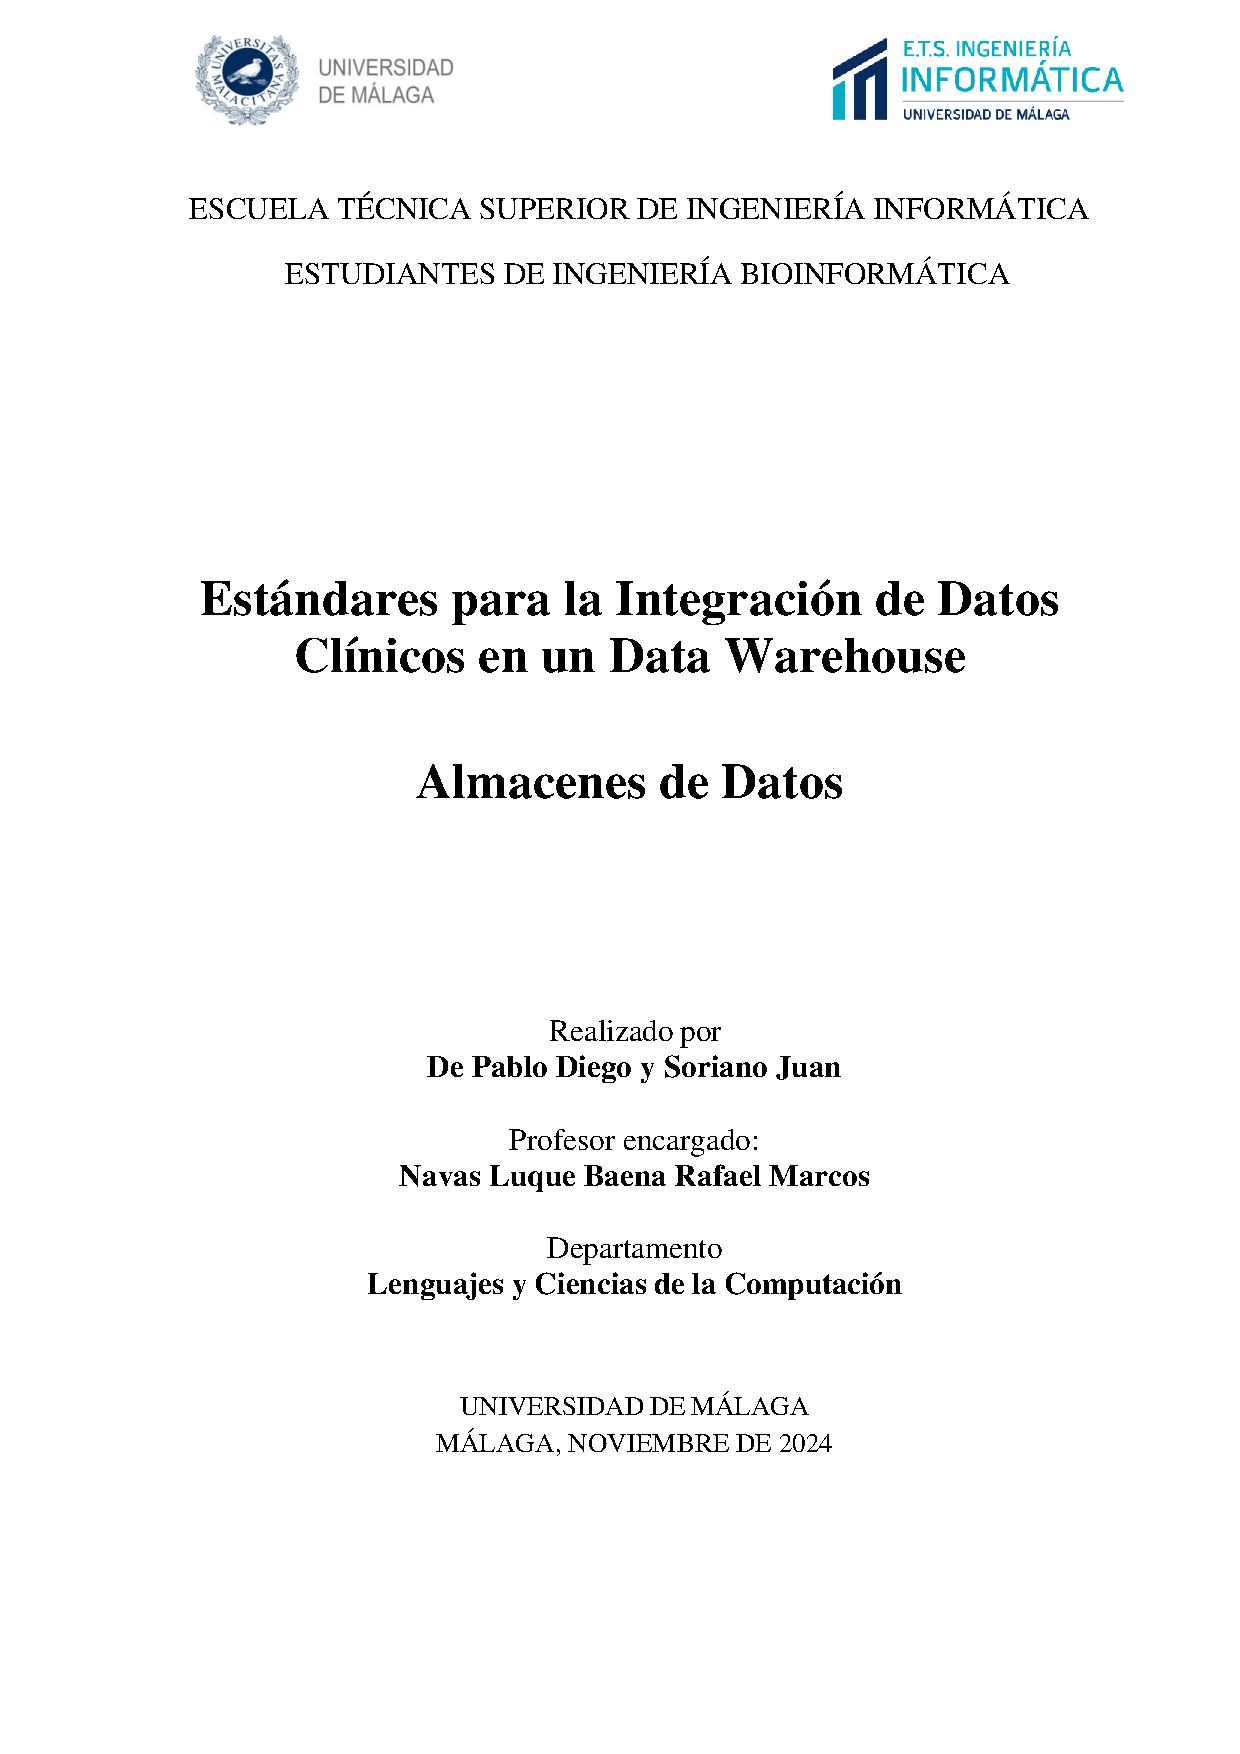
\includepdf[noautoscale=true, width=\paperwidth]{title.pdf}
	
	%%%%%%%%%%%%%%%%%%%%%%%%%%%%%%%%%%%%%%%%%%%%%%%%%%%%%%%%%%%%%%%%%%%%%%%%%%%
	
	% Índice automático
	\tableofcontents
	\newpage
	
	% Sections
	\section{Introducción a la Integración de Datos Clínicos en un Data Warehouse}
	Describe el propósito y la importancia de la integración de datos clínicos en un contexto centralizado.
	
	\section{Fundamentos y Conceptos Clave de los Data Warehouses en el Ámbito Clínico}
	
	Un \textbf{data warehouse} (almacén de datos) es un sistema diseñado para la recolección, almacenamiento y análisis de grandes volúmenes de datos provenientes de diversas fuentes. Esta plataforma reúne diversas tecnologías y componentes aprovechando al máximo los datos. Permite almacenar una gran cantidad de datos, así como también su tratamiento y análisis. El objetivo es \textbf{transformar los datos brutos en informaciones útiles}, y volverlos disponibles y accesibles para los usuarios \cite{Portal2017}.
	
	La función de un data warehouse es actuar como un repositorio centralizado donde se recopilan datos de múltiples fuentes, como bases de datos transaccionales, sistemas ERP o archivos externos. Estos datos pueden ser estructurados (tablas relacionales), semiestructurados (como archivos XML o JSON) o no estructurados (texto libre, imágenes)\cite{Portal2017}.
	
	Una vez los datos llegan al data warehouse, pasan por un proceso de \textbf{ETL} (Extracción, Transformación y Carga), donde son limpiados, organizados y transformados para su análisis. Los usuarios pueden acceder a estos datos mediante herramientas de \textbf{Business Intelligence} (BI), consultas SQL o visualizaciones interactivas.
	
	Al centralizar la información, las organizaciones obtienen una visión completa y coherente de sus datos, lo que facilita la toma de decisiones basadas en hechos. Además, el data warehouse habilita técnicas de \textbf{data mining}, que permiten descubrir patrones ocultos y tendencias para mejorar estrategias comerciales o de operación\cite{kimball2013}.
	
	En el ámbito clínico, los \textbf{sistemas de información sanitaria} (SIS) recopilan volúmenes crecientes de datos provenientes de la atención médica rutinaria. Esta fuente de \textbf{datos del mundo real} (RWD, por sus siglas en inglés) ofrece un gran potencial para mejorar la calidad de la atención médica. Por un lado, estos datos aportan beneficios directos al paciente —usos primarios— al ser fundamentales para el desarrollo de la medicina personalizada. Al mismo tiempo, brindan beneficios indirectos —usos secundarios— al acelerar y mejorar la generación de conocimiento sobre patologías, condiciones de uso de productos y tecnologías sanitarias, así como la evaluación de su seguridad, eficacia y utilidad en la práctica diaria. Estos datos también son útiles para medir el impacto organizacional de las tecnologías de salud. El \textbf{manejo eficiente de grandes volúmenes de datos} a través de un data warehouse es una de las ventajas más importantes que permite maximizar el uso de esta información para mejorar los resultados en salud.
	
	
	\subsection{Fases del Flujo de Datos en un Clinical Data Warehouse (CDW)}
	
	El \textbf{Clinical Data Warehouse (CDW)} es una infraestructura que permite consolidar datos provenientes de uno o varios \textbf{Sistemas de Información Médica} (HIS, por sus siglas en inglés) en formatos homogéneos, independientemente del marco organizativo o del origen de los datos. Esta estructura es esencial para facilitar la reutilización de la información en diversos contextos como la gestión, la investigación y la atención médica. \cite{doutreligne2023}
	
	La \textbf{Figura \ref{fig:Flujo}} ilustra las cuatro fases clave del flujo de datos que conforman un CDW, desde la recopilación de las fuentes originales hasta los usos finales, destacando el proceso de transformación e integración de los datos.
	
	\begin{figure}[h!]
		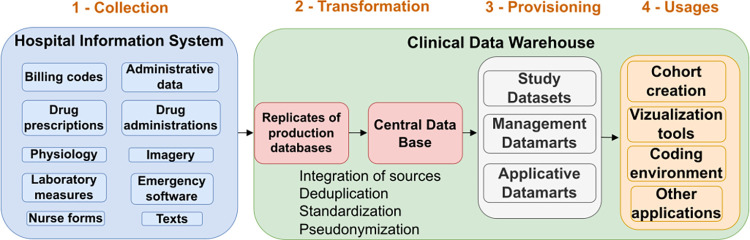
\includegraphics[width=1\textwidth]{image/Flujo.jpg}
		\caption{Cuatro pasos del flujo de datos del Sistema de Información Hospitalaria: (1) recopilación, (2) transformaciones y (3) aprovisionamiento. CDW, almacén de datos clínicos.\cite{doutreligne2023}}
		\label{fig:Flujo}
	\end{figure}
	
	\begin{enumerate}
		\item \textbf{Recopilación (Collection)}  
		La primera fase consiste en extraer los datos de las distintas fuentes que componen el HIS. Estas fuentes pueden incluir datos administrativos, prescripciones de medicamentos, mediciones fisiológicas, resultados de laboratorio, formularios de enfermería, entre otros. El objetivo principal es capturar la mayor variedad de datos posibles para que el CDW sirva como un repositorio central que refleje de manera precisa la información clínica almacenada en los sistemas hospitalarios. Cada una de estas fuentes puede estar almacenada en diferentes formatos, lo que subraya la necesidad de normalización en las fases posteriores.
		
		\item \textbf{Transformación (Transformation)}  
		Tras la recopilación, los datos pasan por un proceso de transformación donde se integran y armonizan para asegurar su coherencia. En esta fase se distinguen varias etapas clave:  
		\begin{itemize}
			\item \textit{Integración de fuentes}: Los datos de diferentes bases son unificados en una base central.  
			\item \textit{Desduplicación de identificadores}: Se eliminan las duplicaciones y se normalizan los identificadores que se puedan repetir en diversas fuentes.  
			\item \textit{Estandarización}: Un modelo de datos único, independiente de los sistemas de origen, asegura que los datos se almacenen y estructuren bajo un esquema común. Este proceso es crucial para asegurar la interoperabilidad y puede incluir la adopción de nomenclaturas estándar como SNOMED CT o LOINC.  
			\item \textit{Pseudonimización}: Con el fin de proteger la privacidad del paciente, los datos sensibles son anonimizados mediante técnicas de pseudonimización, eliminando o codificando cualquier información directamente identificativa.
		\end{itemize}
		
		\item \textbf{Provisión (Provisioning)}  
		Una vez que los datos han sido transformados, se almacenan en una base central y se dividen en subconjuntos específicos o \textit{datamarts}, que permiten su reutilización tanto en usos primarios como secundarios. Estos \textit{datamarts} pueden estar orientados a diferentes objetivos, como estudios específicos, gestión administrativa o aplicaciones clínicas. El uso de \textit{datamarts} especializados optimiza el acceso a los datos y facilita la creación de \textit{cohortes}, la utilización de \textit{herramientas de visualización}, así como el acceso a un \textit{entorno de codificación} y otras aplicaciones.
		
		\item \textbf{Usos (Usages)}  
		En esta última fase, los usuarios del CDW pueden acceder a los datos ya procesados y almacenados en los \textit{datamarts} a través de aplicaciones y herramientas especializadas. Los principales usos incluyen:
		\begin{itemize}
			\item \textit{Creación de cohortes}: Selección de subpoblaciones específicas basadas en criterios clínicos para su análisis en estudios de investigación.  
			\item \textit{Herramientas de visualización}: Plataformas que permiten explorar los datos mediante gráficos, tablas y otras representaciones visuales para facilitar el análisis.  
			\item \textit{Entornos de codificación}: Espacios diseñados para realizar análisis avanzados y procesar los datos de manera eficiente mediante técnicas de \textit{machine learning} o análisis estadístico.  
			\item \textit{Otras aplicaciones}: Los datos también pueden ser reutilizados en diversas aplicaciones, desde la mejora de procesos clínicos hasta la evaluación de nuevas tecnologías o tratamientos.
		\end{itemize}
	\end{enumerate}
	
	
	
	\subsection{Relevancia en el Manejo de Datos de Salud}

	La relevancia de los data warehouses en el manejo de datos de salud radica en su capacidad para ofrecer un enfoque holístico y basado en datos en la atención médica. Algunos beneficios clave incluyen\cite{turcan2022}:
	
	\begin{itemize}
		\item \textbf{Mejora en la Toma de Decisiones:} Los data warehouses permiten a los clínicos acceder a datos integrados y actualizados, lo que mejora la calidad de la atención al paciente. Con datos precisos y en tiempo real, los médicos pueden tomar decisiones informadas sobre diagnósticos y tratamientos.
		
		\item \textbf{Apoyo a la Investigación:} Los investigadores pueden utilizar los datos almacenados en un data warehouse para realizar estudios epidemiológicos, ensayos clínicos y análisis de resultados. La posibilidad de acceder a grandes volúmenes de datos clínicos facilita la identificación de tendencias y patrones que pueden mejorar la atención médica.
		
		\item \textbf{Análisis Predictivo:} Mediante técnicas de análisis de datos y minería de datos, los data warehouses permiten realizar predicciones sobre eventos futuros, como la probabilidad de readmisión de un paciente o la identificación de brotes de enfermedades. Esto puede resultar en intervenciones tempranas y mejor planificación de recursos.
		
		\item \textbf{Interoperabilidad:} La integración de datos de múltiples fuentes a través de un data warehouse fomenta la interoperabilidad entre sistemas de información de salud. Esto es fundamental en un entorno donde diferentes proveedores de atención médica utilizan diferentes sistemas y estándares para almacenar datos.
		
		\item \textbf{Cumplimiento Normativo y Reporte:} Los data warehouses permiten a las organizaciones de salud cumplir con las normativas y estándares de reporte, facilitando la generación de informes para entidades regulatorias y aseguradoras. Esto no solo mejora la transparencia, sino que también ayuda a las organizaciones a obtener financiamiento y soporte.
		
	\end{itemize}


	
	\section{Estándares de Interoperabilidad en Datos Clínicos}
	Detalla los principales estándares (HL7, FHIR, SNOMED CT, LOINC) y cómo facilitan la integración y el intercambio de datos clínicos entre sistemas.
	
	\section{Arquitectura del Data Warehouse Clínico}
	
	La arquitectura de un \textbf{data warehouse clínico} es fundamental para el análisis de datos de salud. Esta arquitectura se compone de varias capas que interactúan entre sí para garantizar que los datos sean accesibles, confiables y utilizables para la toma de decisiones clínicas. A continuación, se explican las capas y los componentes esenciales de esta arquitectura
	
	\subsection{Capas de la Arquitectura del Data Warehouse}

	La \textbf{Figura \ref{fig:Arqui}} ilustra una simplificación de la arquitectura típica de un data warehouse clínico se puede dividir en las siguientes capas:
	
	
	\begin{figure}[h!]
		\centering % Acentúa la figura al centro
		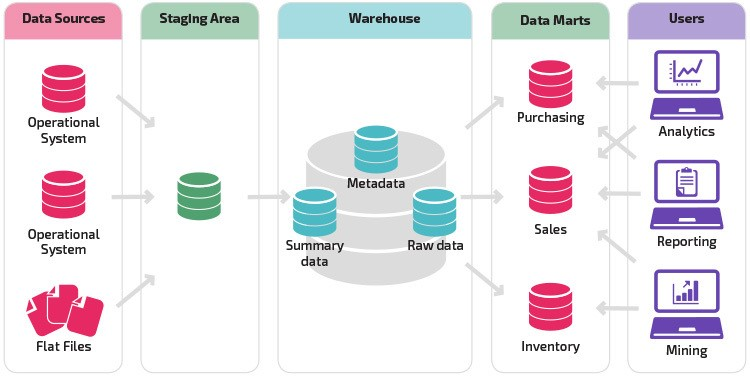
\includegraphics[width=1\textwidth]{image/Arquitectura.jpg}
		\caption{5 puntos de la arquitectura del Data Warehouse: (1) Fuentes de Datos, (2) Carga (ETL), (3) Warehouse o almacenamiento, (4) Procesamiento y (5) Presentación.} % Asegúrate de cerrar el caption correctamente
		\label{fig:Arqui}
	\end{figure}
	
	
	\begin{itemize}
		\item \textbf{Capa de Fuentes de Datos:} Esta es la base del data warehouse y está compuesta por diversas fuentes de datos clínicas, como lo pueden ser:
		\begin{itemize}
			\item \textit{Registros Electrónicos de Salud (EHR):} Documentos digitales que contienen información sobre la salud de los pacientes.
			\item \textit{Sistemas de Información de Salud (HIS):} Plataformas que integran y gestionan datos clínicos y administrativos.
			\item \textit{Sistemas de Laboratorio:} Sistemas que gestionan datos de pruebas y resultados de laboratorio.
			\item \textit{Dispositivos de Monitoreo:} Equipos que recogen datos de salud en tiempo real, como monitores de signos vitales.
		\end{itemize}
		
		\item \textbf{Capa de Extracción, Transformación y Carga (ETL):} Esta capa es crucial para preparar los datos antes de ser almacenados en el data warehouse. Las actividades incluyen:
		\begin{itemize}
			\item \textit{Extracción:} Obtención de datos desde las diferentes fuentes mencionadas.
			\item \textit{Transformación:} Normalización, limpieza y enriquecimiento de datos para asegurar la calidad y consistencia. Esto puede incluir la conversión de formatos, eliminación de duplicados y la integración de datos de distintas fuentes.
			\item \textit{Carga:} Inserción de los datos transformados en el repositorio del data warehouse.
		\end{itemize}
		
		\item \textbf{Capa de Almacenamiento:} En esta capa se encuentran los datos organizados y estructurados, donde se utilizan diferentes modelos de datos:
		\begin{itemize}
			\item \textit{Modelo Estrella:} Un esquema que organiza los datos en una tabla de hechos central conectada a varias tablas de dimensiones. Este modelo facilita consultas rápidas y análisis.
			\item \textit{Modelo Copo de Nieve:} Una variante del modelo estrella, donde las tablas de dimensiones están normalizadas para reducir la redundancia de datos.
			\item \textit{Data Mart:} Subconjuntos de un data warehouse que están diseñados para un área específica, como el manejo de enfermedades crónicas o análisis de laboratorio.
		\end{itemize}
		
		\item \textbf{Capa de Procesamiento:} Esta capa se encarga de procesar y analizar los datos almacenados. Se puede incluir:
		\begin{itemize}
			\item \textit{Minería de Datos:} Técnicas que permiten descubrir patrones, correlaciones y tendencias en grandes volúmenes de datos clínicos.
			\item \textit{Análisis Predictivo:} Modelos estadísticos y algoritmos que utilizan datos históricos para predecir eventos futuros, como la probabilidad de enfermedades.
			\item \textit{Informes y Dashboards:} Herramientas que permiten a los usuarios visualizar datos y métricas a través de gráficos interactivos y resúmenes visuales.
		\end{itemize}
		
		\item \textbf{Capa de Presentación:} Esta capa proporciona acceso a los datos a los usuarios finales. Los usuarios pueden interactuar con los datos a través de:
		\begin{itemize}
			\item \textit{Interfaces de Usuario:} Aplicaciones web o móviles que permiten a los profesionales de la salud consultar y analizar datos de manera intuitiva.
			\item \textit{Herramientas de BI (Business Intelligence):} Software que ayuda en la toma de decisiones a través de la creación de informes, análisis de tendencias y generación de métricas de rendimiento.
		\end{itemize}
	\end{itemize}
	
	
	Además de la arquitectura, también se deben considerar otros componentes clave para asegurar la calidad y eficiencia de un data warehouse clínico. Esto incluye la gobernanza de datos, que establece políticas para garantizar la calidad y privacidad de la información; la gestión de calidad de datos, que utiliza herramientas para asegurar la precisión y completitud de los datos mediante limpieza y monitoreo; la seguridad de datos, que protege la confidencialidad e integridad de la información a través de autenticación y cifrado; la interoperabilidad, que permite el intercambio efectivo de datos entre sistemas mediante estándares como HL7 y FHIR; y el mantenimiento y soporte, que asegura la continuidad operativa mediante actualizaciones y soporte técnico.
	
	
	\section{Proceso ETL para la Integración de Datos Clínicos}
	Explica las etapas de Extracción, Transformación y Carga (ETL) para normalizar y consolidar datos clínicos de diversas fuentes.
	
	\section{Beneficios de la Integración de Datos Clínicos}
	Enumera y detalla los beneficios clave de un data warehouse clínico: mejora en la toma de decisiones, apoyo a la investigación, análisis predictivo, etc.
	
	\section{Relación con el Curso de Almacenes de Datos}
	Analiza cómo los conceptos de la asignatura, como modelado de datos, arquitecturas de data warehouse y técnicas de ETL, se aplican en el desarrollo de un data warehouse clínico.
	
	\section{Ejemplos de Uso y Casos Prácticos de Integración de Datos Clínicos}
	Proporciona ejemplos de aplicación práctica, simulando la integración de datos de un sistema de EHR en un data warehouse usando algún estándar.
	
	\section{Conclusiones y Perspectivas Futuras en la Integración de Datos Clínicos}
	Ofrece un resumen de los puntos más importantes y discute posibles desarrollos futuros en la interoperabilidad y los data warehouses clínicos.
	
	%%%%%%%%%%%%%%%%%%%%%%%%%%%%%%%%%%%%%%%%%%%%%%%%%%%%%%%%%%%%%%%%%%%%%%%%%%%
	\section{Bibliografía}
	\printbibliography
	
	%% Back Cover
	
\includepdf[noautoscale=true, width=\paperwidth]{backcover.pdf}
	
\end{document}